%-------------------------------------------------------------
\documentclass{beamer}
\usepackage[utf8]{inputenc}
\usepackage{hyperref}
\usepackage[T1]{fontenc}
\usepackage{tikz}

\usepackage{latexsym,xcolor,multicol,booktabs,calligra}
\usepackage{amsmath,amssymb,BOONDOX-cal,bm}	
\usepackage{graphicx,pstricks,stackengine}      


\author{Michael John Curry}
\title{HDR Image Construction from a LDR Dataset for Deep Learning}
\institute{SUNY New Paltz} 


\usepackage{Wue}

\def\cmd#1{\texttt{\color{red}\footnotesize $\backslash$#1}}
\def\env#1{\texttt{\color{blue}\footnotesize #1}}

\newtheorem{thm}{Theorem}[theorem]


%—-------------------------------------------------------------

\begin{document}
	\begin{frame}
    \titlepage
    \end{frame}

	
	\begin{frame}
		\tableofcontents[sectionstyle=show,subsectionstyle=show/shaded/hide,subsubsectionstyle=show/shaded/hide]
	\end{frame}
	
		%—------------------------------------------------------
	\section{Data Augmentation}
	    %\subsection{}
		    \begin{frame}
			    \begin{itemize} 
			    \item 
			    The best way to improve the performance of a machine learning model is to train it on more data. The more examples the model has to learn from, the better it will be able to recognize which differences in images matter and which do not.
                \end{itemize}
                \begin{itemize}
                \item 
			    One easy way of getting more data is to use the data you already have. If we can transform the images in our dataset in ways that preserve the class, we can teach our classifier to ignore those kinds of transformations.  
                \end{itemize}
                 \begin{itemize}
                \item 
			    Some examples are rotation, translation, flipping, brightness, and contrast. 
                \end{itemize}
		    \end{frame}
		    
		    \begin{frame}
		        \begin{itemize}
		        \item 
		        Are there other methods to increase the amount of data contained in an image? 
		        \end{itemize}
		    \end{frame}
	
		
	
	%—------------------------------------------------------
	\section{High-Dynamic-Range (HDR) Images}
	    %\subsection{}
		    \begin{frame}
			    \begin{itemize} 
			    \item 
			    High-dynamic-range (HDR) imaging, an important field in image
                processing, computer graphics/vision, and photography,  
                is a technique that allows a greater dynamic range of exposures
                than traditional imaging techniques. It aims to accurately represent
                a wide range of intensity levels captured in real scenes, ranging
                from sunlight to shadows.
			  
                \end{itemize}
		    \end{frame}
		    
		    \begin{frame}
		        \begin{itemize}
		        \item 
		        Conventional HDR imaging mainly uses special HDR cameras to capture HDR images.  These cameras are prohibitively expensive for
                general users. 
		        \end{itemize}
		    \end{frame}
	
	%-------------------------------------------------------	
	\section{Low-Dynamic-Range (LDR) Images}
	    %\subsection{}
		    \begin{frame}
			    \begin{itemize}
			    \item 
			     All images captured by consumer, pro-consumer, and most professional cameras.  These images make up the vast majority of the images captured each day.  
                \end{itemize}
		    \end{frame}
		    \begin{frame}
			    \begin{itemize}
			    \item 
			    A method to reconstruct HDR images from the visual content
                captured by low-dynamic-range (LDR) cameras using specially designed algorithms.
                
                \item
                One common approach is to capture multiple exposures of a scene and then combine them.  
			    \end{itemize}	
		    \end{frame}
		    \begin{frame}
		    \begin{itemize}
		        \item 
		        If the scene was not originally captured with multiple exposures, are there ways to bring back the lost information?
		        
		    \end{itemize}
		        
		    \end{frame}
		    
		    \begin{frame}
		    \begin{itemize}
		        \item 
		        GAN networks, Deep neutral networks, and virtual environment rendering techniques are all used to create a HDR image from a single LDR capture.  
		        
		        \item
		        All these approaches are computationally expensive. 
             \end{itemize}
		        
		    \end{frame}
		    
		    \begin{frame}
		    \begin{itemize}
		        \item
		        Is there a naive approach?
		    \end{itemize}
		        
		    \end{frame}
	
	%-----------------------------------------------------
	\section{HDR Image Construction from a LDR Dataset}
	    %\subsection{}
	
	\begin{frame}{Original Image}
 
		\begin{columns}[T]
			\begin{column}<0->{.5\textwidth}
				\begin{figure}[thpb]
					\centering
					\resizebox{1.25\linewidth}{!}{
						\includegraphics{Original.png}
					}
					%	\includegraphics[scale=1.0]{figurefile}
					\caption{Original Image}
					\label{fig:1}
				\end{figure}
			\end{column}%
			\hfill%
			\begin{column}<0->{.3\textwidth}
				\centering
			    \begin{itemize} 
			    \item Data loss in both Highlights and Shadows
			    \end{itemize}
		   
			\end{column}
		\end{columns}
	\end{frame}
	
		\begin{frame}{Multiply Blending Mode}
 
		\begin{columns}[T]
			\begin{column}<0->{.5\textwidth}
				\begin{figure}[thpb]
					\centering
					\resizebox{1.25\linewidth}{!}{
						\includegraphics{Multiply.png}
					}
					%	\includegraphics[scale=1.0]{figurefile}
					\caption{Multiply}
					\label{fig:1}
				\end{figure}
			\end{column}%
			\hfill%
			\begin{column}<0->{.35\textwidth}
				


			    \begin{itemize} 
			    \item All pixel luminosity values in the lightest third have Multiply blending mode applied. 
			    \begin{align*} f(a,b) = ab \end{align*}
			    
			    \end{itemize}
		        
			\end{column}
		\end{columns}
	\end{frame}
	
	\begin{frame}{Screen Blending Mode}
 
		\begin{columns}[T]
			\begin{column}<0->{.5\textwidth}
				\begin{figure}[thpb]
					\centering
					\resizebox{1.25\linewidth}{!}{
						\includegraphics{Screen.png}
					}
					%	\includegraphics[scale=1.0]{figurefile}
					\caption{Multiply}
					\label{fig:1}
				\end{figure}
			\end{column}%
			\hfill%
			\begin{column}<0->{.35\textwidth}
				


			    \begin{itemize} 
			    \item All pixel luminosity values in the darkest third have Screen blending mode applied. 
			    \begin{align*} f(a,b) = 1-(1-a)(1-b) \end{align*}
			    
			    \end{itemize}
		        
			\end{column}
		\end{columns}
	\end{frame}
	
		\begin{frame}{Combine all three images}
 
		\begin{columns}[T]
			\begin{column}<0->{.5\textwidth}
				\begin{figure}[thpb]
					\centering
					\resizebox{1.25\linewidth}{!}{
						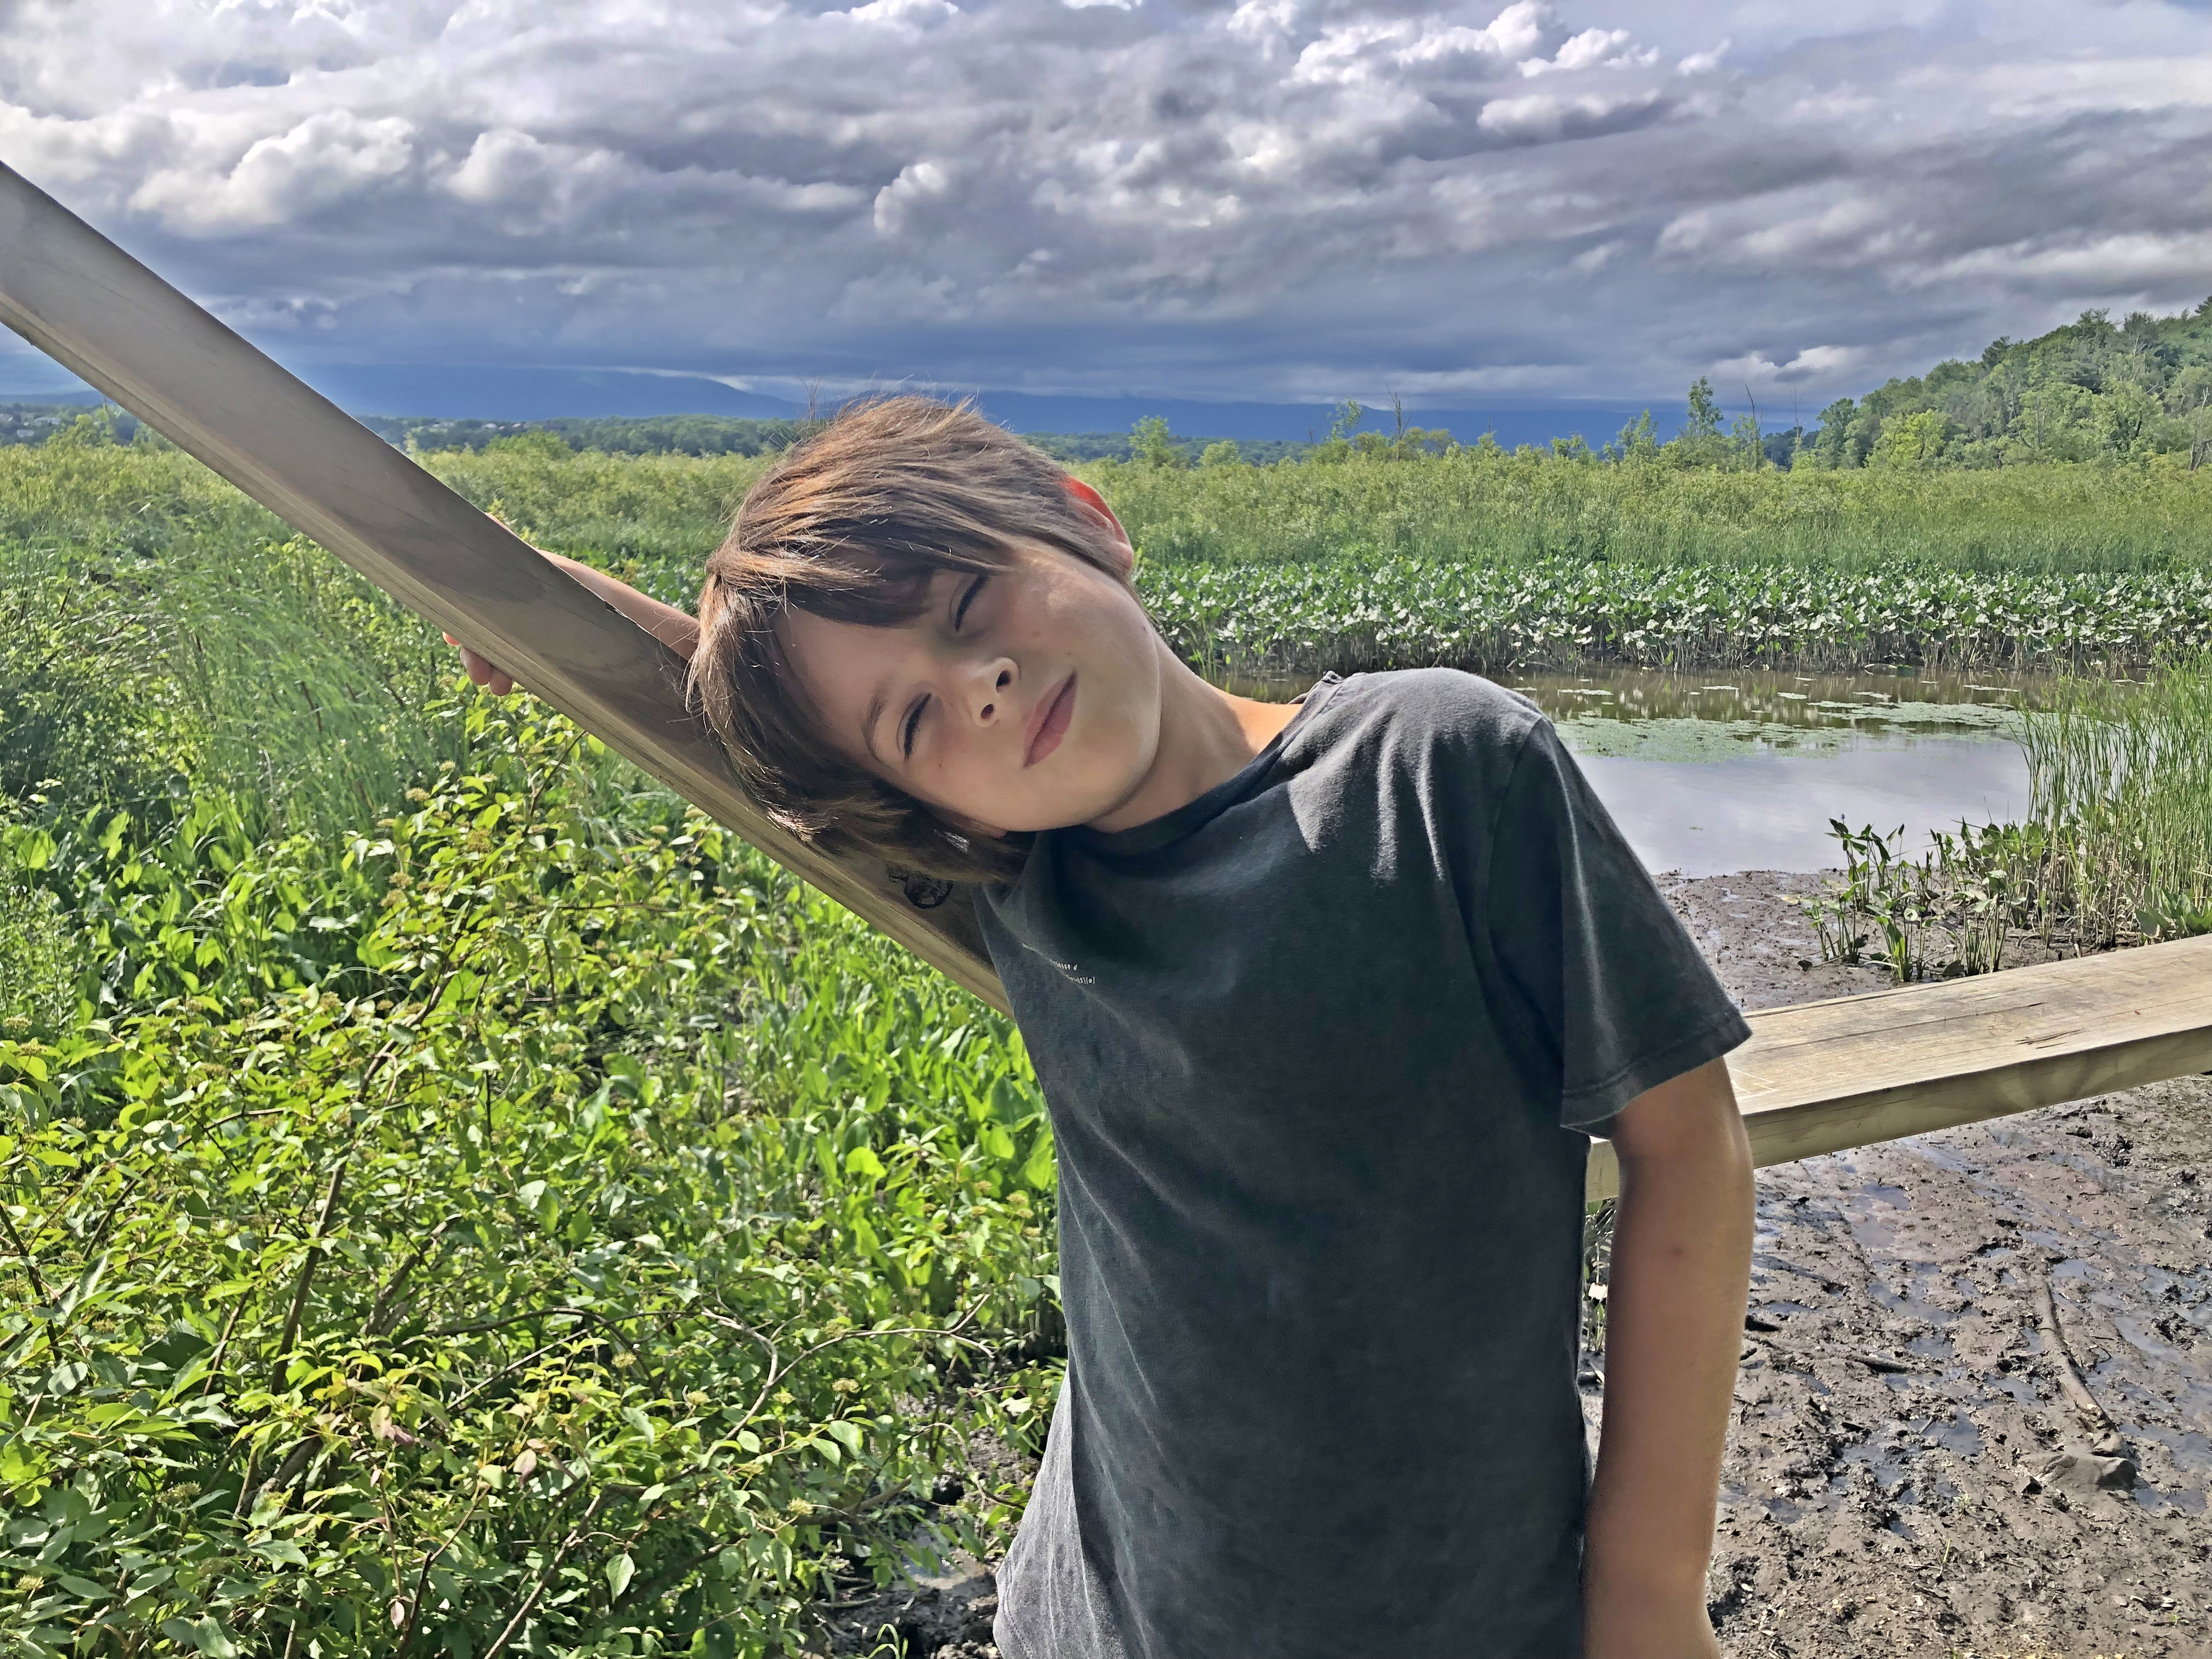
\includegraphics{Screen_Multiply.png}
					}
					%	\includegraphics[scale=1.0]{figurefile}
					\caption{Combined}
					\label{fig:1}
				\end{figure}
			\end{column}%
			\hfill%
			\begin{column}<0->{.3\textwidth}
				\centering
			    \begin{itemize} 
			    \item 
			    All three images are stacked.
			    \end{itemize}
		   
			\end{column}
		\end{columns}
	\end{frame}
	
	\begin{frame}
			    \begin{itemize} 
			    
			     \item 
			    Highlight information is taken from the image with the Multiply blending mode applied. 
			    \item 
			    Mid-tone information is taken from the original unprocessed image.
			    \item
			    Shadow information is taken from the image with the Screen blending mode applied. 
			    \end{itemize}
			    \end{frame}


	
	%-------------------------------------------------


	%----------------------------------------------
%	\section{References}
%		
%		\begin{frame}[allowframebreaks]
%			\bibliographystyle{unsrt}
%			\bibliography{Bibliography.bib}	
%		\end{frame}
%%
	%-------------------------------------------
%	\begin{frame}
%		\begin{center}
%			{\Huge \emph {\textrm{Thank  ~you!}}}
%		\end{center}
%	\end{frame}

\end{document}